\documentclass[notes,11pt, aspectratio=169]{beamer}

\usepackage{pgfpages}
% These slides also contain speaker notes. You can print just the slides,
% just the notes, or both, depending on the setting below. Comment out the want
% you want.
\setbeameroption{hide notes} % Only slide
%\setbeameroption{show only notes} % Only notes
%\setbeameroption{show notes on second screen=right} % Both

\usepackage{helvet}
\usepackage[default]{lato}
\usepackage{array}
\usepackage{tgbonum}

\usepackage{tikz}
\usepackage{verbatim}
\setbeamertemplate{note page}{\pagecolor{yellow!5}\insertnote}
\usetikzlibrary{positioning}
\usetikzlibrary{snakes}
\usetikzlibrary{calc}
\usetikzlibrary{arrows}
\usetikzlibrary{decorations.markings}
\usetikzlibrary{shapes.misc}
\usetikzlibrary{matrix,shapes,arrows,fit,tikzmark}
\usepackage{amsmath}
\usepackage{mathpazo}
\usepackage{hyperref}
\usepackage{lipsum}
\usepackage{multimedia}
\usepackage{graphicx}
\usepackage{multirow}
\usepackage{graphicx}
\usepackage{dcolumn}
\usepackage{bbm}
\newcolumntype{d}[0]{D{.}{.}{5}}

\usepackage{changepage}
\usepackage{appendixnumberbeamer}
\newcommand{\beginbackup}{
   \newcounter{framenumbervorappendix}
   \setcounter{framenumbervorappendix}{\value{framenumber}}
   \setbeamertemplate{footline}
   {
     \leavevmode%
     \hline
     box{%
       \begin{beamercolorbox}[wd=\paperwidth,ht=2.25ex,dp=1ex,right]{footlinecolor}%
%         \insertframenumber  \hspace*{2ex} 
       \end{beamercolorbox}}%
     \vskip0pt%
   }
 }
\newcommand{\backupend}{
   \addtocounter{framenumbervorappendix}{-\value{framenumber}}
   \addtocounter{framenumber}{\value{framenumbervorappendix}} 
}


\usepackage{graphicx}
\usepackage[space]{grffile}
\usepackage{booktabs}
\newcommand\independent{\protect\mathpalette{\protect\independenT}{\perp}}
\def\independenT#1#2{\mathrel{\rlap{$#1#2$}\mkern2mu{#1#2}}}
\DeclareMathOperator{\Supp}{Supp}

% These are my colors -- there are many like them, but these ones are mine.
\definecolor{blue}{RGB}{0,114,178}
\definecolor{red}{RGB}{213,94,0}
\definecolor{yellow}{RGB}{240,228,66}
\definecolor{green}{RGB}{0,158,115}

\hypersetup{
  colorlinks=false,
  linkbordercolor = {white},
  linkcolor = {blue}
}


%% I use a beige off white for my background
\definecolor{MyBackground}{RGB}{255,253,218}

%% Uncomment this if you want to change the background color to something else
%\setbeamercolor{background canvas}{bg=MyBackground}

%% Change the bg color to adjust your transition slide background color!
\newenvironment{transitionframe}{
  \setbeamercolor{background canvas}{bg=yellow}
  \begin{frame}}{
    \end{frame}
}

\setbeamercolor{frametitle}{fg=blue}
\setbeamercolor{title}{fg=black}
\setbeamertemplate{footline}[frame number]
\setbeamertemplate{navigation symbols}{} 
\setbeamertemplate{itemize items}{-}
\setbeamercolor{itemize item}{fg=blue}
\setbeamercolor{itemize subitem}{fg=blue}
\setbeamercolor{enumerate item}{fg=blue}
\setbeamercolor{enumerate subitem}{fg=blue}
\setbeamercolor{button}{bg=MyBackground,fg=blue,}



% If you like road maps, rather than having clutter at the top, have a roadmap show up at the end of each section 
% (and after your introduction)
% Uncomment this is if you want the roadmap!
% \AtBeginSection[]
% {
%    \begin{frame}
%        \frametitle{Roadmap of Talk}
%        \tableofcontents[currentsection]
%    \end{frame}
% }
\setbeamercolor{section in toc}{fg=blue}
\setbeamercolor{subsection in toc}{fg=red}
\setbeamersize{text margin left=1em,text margin right=1em} 

\newenvironment{wideitemize}{\itemize\addtolength{\itemsep}{10pt}}{\enditemize}

\usepackage{environ}
\NewEnviron{videoframe}[1]{
  \begin{frame}
    \vspace{-8pt}
    \begin{columns}[onlytextwidth, T] % align columns
      \begin{column}{.70\textwidth}
        \begin{minipage}[t][\textheight][t]
          {\dimexpr\textwidth}
          \vspace{8pt}
          \hspace{4pt} {\Large \sc \textcolor{blue}{#1}}
          \vspace{8pt}
          
          \BODY
        \end{minipage}
      \end{column}%
      \hfill%
      \begin{column}{.38\textwidth}
        \colorbox{green!20}{\begin{minipage}[t][1.2\textheight][t]
            {\dimexpr\textwidth}
            Face goes here
          \end{minipage}}
      \end{column}%
    \end{columns}
  \end{frame}
}

\title[]{\textcolor{blue}{Canonical Research Designs I:\\ Difference-in-Differences II:\\
  Event Studies, Synthetic Control, and Synthetic DinD}}
\author[PGP]{}
\institute[FRBNY]{\small{\begin{tabular}{c}
  Paul Goldsmith-Pinkham  \\
\end{tabular}}}

\date{\today}

\begin{document}

%%% TIKZ STUFF
\tikzset{   
        every picture/.style={remember picture,baseline},
        every node/.style={anchor=base,align=center,outer sep=1.5pt},
        every path/.style={thick},
        }
\newcommand\marktopleft[1]{%
    \tikz[overlay,remember picture] 
        \node (marker-#1-a) at (-.3em,.3em) {};%
}
\newcommand\markbottomright[2]{%
    \tikz[overlay,remember picture] 
        \node (marker-#1-b) at (0em,0em) {};%
}
\tikzstyle{every picture}+=[remember picture] 
\tikzstyle{mybox} =[draw=black, very thick, rectangle, inner sep=10pt, inner ysep=20pt]
\tikzstyle{fancytitle} =[draw=black,fill=red, text=white]
%%%% END TIKZ STUFF

% Title Slide
\begin{frame}
\maketitle
\end{frame}

\begin{frame}{Today's Topics}
  \begin{wideitemize}
  \item Today, touching on two (related) topics
  \item First, finishing conversation on standard diff-in-diff,
    focusing on \emph{event studies}
    \begin{itemize}
    \item How do event studies generate a counteractual control unit
    \item Issue: dynamic effects \textbf{plus} staggered timing \textbf{plus} heterogeneity
    \end{itemize}
  \item Second, discuss synthetic control (and dind) methods
    \begin{itemize}
    \item Not completely new methods, but big upswing in research
    \end{itemize}
  \end{wideitemize}
\end{frame}

\begin{frame}{Event study}
  \begin{columns}[T] % align columns
    \begin{column}{0.6\textwidth}
      \begin{wideitemize}
      \item Two important cases with these staggered timing dind (event studies)
        \begin{itemize}
        \item There exists a never-treated group who is a potential control group
        \item Everyone is treated eventually  (No group is a ``pure control'')
        \end{itemize}
      \item The older approach to estimate this model was:
        \begin{equation*}
          Y_{it} = \alpha_{i} + \gamma_{t} + \sum_{s = L_{0}, s\not=-1}^{L_{1}}1(t-T_{i} = s)\mu_{s}
        \end{equation*}
      \item Without a true control group, can't have both time
        fe, unit fe, and the full set of relative effects
        \vspace{-15pt}
      \item Need to exclude both the baseline period AND at least
        some periods outside the treatment window
      \end{wideitemize}
      \end{column}%
      \hfill%
      \begin{column}{.4\textwidth}
        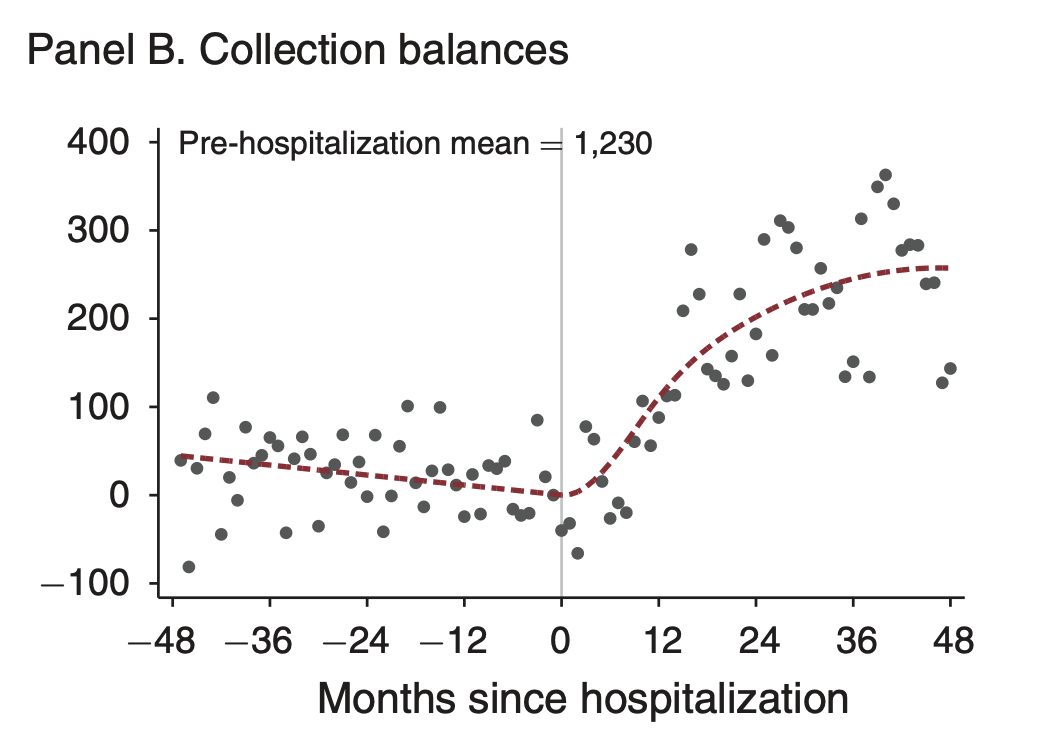
\includegraphics[width=\linewidth]{images/noto1.png}\\
        \begin{itemize}
        \item Dobkin et al. (2018)
        \item Comparison is between those not yet hospitalized and those hospitalized
        \end{itemize}
      \end{column}%
    \end{columns}
  \end{frame}

\begin{frame}{Event study continued}
  \begin{wideitemize}
  \item The necessary assumptions are the same (or similar) what we discussed last class
  \item Parallel trends
      \begin{equation}
        E(Y_{i,t}(\infty) - Y_{i,t'}(\infty) | G_{i} = g) =       E(Y_{i,t}(\infty) - Y_{i,t'}(\infty) | G_{i} = g) , \forall g, g', \text{and} t, t'
    \end{equation}
  \item Turns out, all of the groups need to be parallel.
  \item That might be a bad assumption (e.g. very far apart from
    one another)
    \begin{itemize}
    \item Can be weakened in some cases, but only partially
    \end{itemize}
  \item No anticipation:
    \begin{equation}
      Y_{it}(g) = Y_{it}(\infty) \forall t < g
    \end{equation}
  \end{wideitemize}    
\end{frame}

\begin{frame}{Contamination Bias in event studies}
  \begin{wideitemize}
    \item Sun and Abraham (2021) show that if the dynamic path of
    treatment is the same across cohorts ($g$), then the coefficient
    from the TWFE model will correctly estimate the period ATT
    $$\tau_{it}(g)  = \sum_{s\geq0}\tau_{s}1(t-g = s)$$
  \item If not, then there is $g$ specific heterogeneity in paths. This creates issues:
    \begin{itemize}
    \item Violate the pre-trend test as the use of ``excluded''
      periods potentially contaminates pre-periods
    \item Mismeasure the dynamic effects
    \item Additional untestable assumptions are required as we allow for more types of heterogeneity      
    \end{itemize}
  \end{wideitemize}
\end{frame}

\begin{frame}{Issues in Diff-in-Diff - Negative Weighting vs. Contamination Bias}
  \begin{wideitemize}
  \item There are two distinct issues in staggered timings:
    \begin{enumerate}
    \item Goodman-Bacon (2021) and others show that the aggregated
      TWFE estimate can put \emph{negative} weight on some treatment
      cohorts, thereby giving nonsensical estimands
    \item Sun and Abraham (2021) and others show that the
      \emph{dynamic} TWFE estimates can be \emph{contaminated} across
      time 
    \end{enumerate}
  \item See discussion in Goldsmith-Pinkham, Hull and Kolesar (2022)
    appendix for analogy to broader linear regression issue
  \item Key point: TWFE linear regression is misspecified 
  \end{wideitemize}
\end{frame}


\begin{frame}{Solutions: Borusyak Hull and Jaravel (2022) Estimator}
  \begin{wideitemize}
  \item Will walk through Sun and Abraham (2021) solution on homework (interacting treatment effects by cohort)
  \item Callaway and Sant'anna (2021) also provided straightforward solution (not using regression)
  \item BHJ impute the counterfactual using the not-yet-treated observations
    \begin{equation}
      Y_{it}(\infty) = \alpha_{i} + \lambda_{t} + \epsilon_{it}
    \end{equation}
  \item Then, we can predict the value for any unit in a time period:
    $\hat{Y}_{i,t}(\infty)$ and proceed accordingly to construct
    measures of group by time period ATT
    ($\mu_{ATT}(g,t) = E( Y_{i,t}(g) - \hat{Y}_{i,t}(\infty) | G_{i} =
    g)$
  \item What is key difference from Callaway and Sant'anna (and why it is more efficient under some settings?)
    \begin{itemize}
    \item Estimation of $\alpha_{i}$ uses all the pre-treatment data, rather than just the period before
    \end{itemize}
  \end{wideitemize}
\end{frame}


\begin{frame}{Aside in event studies}
  \begin{columns}[T] % align columns
    \begin{column}{0.5\textwidth}
  \begin{wideitemize}
  \item A key factor in how you construct your counterfactual (and
    what assumptions you find plausible) are a function of how far
    into the future you want to estimate outcomes
  \item An extremely short-run counterfactual could potentially just be a linear extrapolation
    \begin{itemize}
    \item This assumes that the underlying model is locally linear,
      rather than globally
    \item Construct a counterfactual from just
      a single time series, but highly non-robust
    \end{itemize}
  \item Example from a robustness check in my own work (Dobbie et al. 2020)
  \end{wideitemize}
    \end{column}%
    \hfill%
    \begin{column}{.5\textwidth}
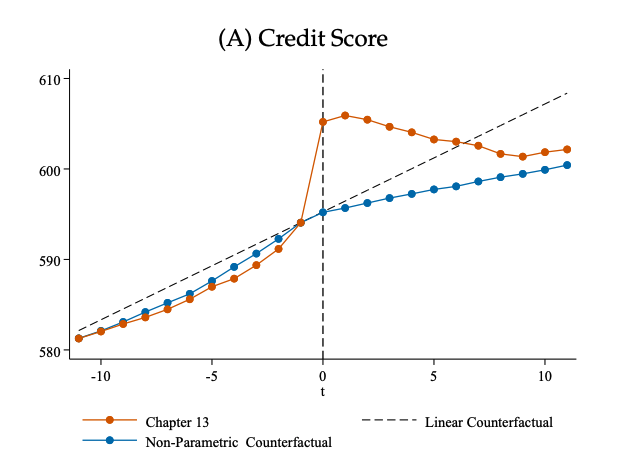
\includegraphics[width=\linewidth]{images/badcredit3.png}        
    \end{column}%
  \end{columns}
\end{frame}

\begin{frame}{Constructing a counterfactual is the key goal}
  \begin{wideitemize}
  \item Issue in event study was the attempt to get a ``free lunch''
    -- we always need a control group
  \item   Think back to cross-sectional setting with ATT
    \begin{itemize}
    \item We always knew $Y_{i}(1)$. Key issue is an estimator for $Y_{i}(0)$.
    \item Event study approaches had issues by ignoring this point and hoping regression would solve problem
    \item Notably, this problem disappears if we have full homogeneity + no anticipation and only exclude pre-periods
    \end{itemize}
  \item Point of emphasis -- we need parallel trends to hold to
    construct a counterfactual in these settings. Why?
    $Y_{jt}(0) - Y_{j,t-1}(0)$ needs to be a good approximator of
    $Y_{i,t}(0) - Y_{i,t-1}(0)$.
    \begin{itemize}
    \item Since we imposed
      $Y_{it} = \alpha_{i} + \gamma_{t} + D_{it}\tau$, the first
      differencing makes them good approximations
    \end{itemize}
  \end{wideitemize}
\end{frame}

\begin{frame}{Generalizing the Dind approach }
  \begin{columns}[T] % align columns
    \begin{column}{0.9\textwidth}
      \begin{wideitemize}
      \item Pivoting slightly: instead of imposing the parallel trends
        assumption directly through the linear model, we could
        construct a combination of units to approximate $Y_{it}(0)$
        \begin{itemize}
        \item This is what one does in the cross-sectional setting with a
          pscore method! E.g. consider the ATT:
          \begin{equation*}
            \tau_{ATT} = \underbrace{Y(1)}_{\text{Fully observed}} - \underbrace{\hat{Y}(0)}_{\text{Constructed}}
          \end{equation*}
        \end{itemize}
      \item How would one pick? Recall that with p-score methods or
        regression, weights effectively reweight based on
        comparability to treated group
        \begin{itemize}
        \item With panel data, can use pre-treatment data to construct
          these weights
        \item This method is known as synthetic control (and its various descendents)
        \end{itemize}
      \end{wideitemize}
    \end{column}%
    \hfill%
    \begin{column}{.5\textwidth}
    \end{column}%
  \end{columns}
\end{frame}


\begin{frame}{Synthetic Control example - (Abadie et al. (2010)) }
  \begin{columns}[T] % align columns
    \begin{column}{0.5\textwidth}
      \begin{wideitemize}
      \item Consider following problem: California bans smoking in 1989. What does that do to smoking?
        \begin{itemize}
        \item Define estimand: $\tau_{ban,CA} = Y_{california, post}(1) - Y_{california, post}(0)$
        \item This is the effect of the \emph{California} smoking ban 
        \item How can we get at it? 
        \end{itemize}
      \item We need a ``synthetic California'' as our control
      \item In an ideal world, the average of the other states would
        work -- however, not clear empirically that they are a good
        counterfactual
      \end{wideitemize}
    \end{column}%
    \hfill%
    \begin{column}{.5\textwidth}
      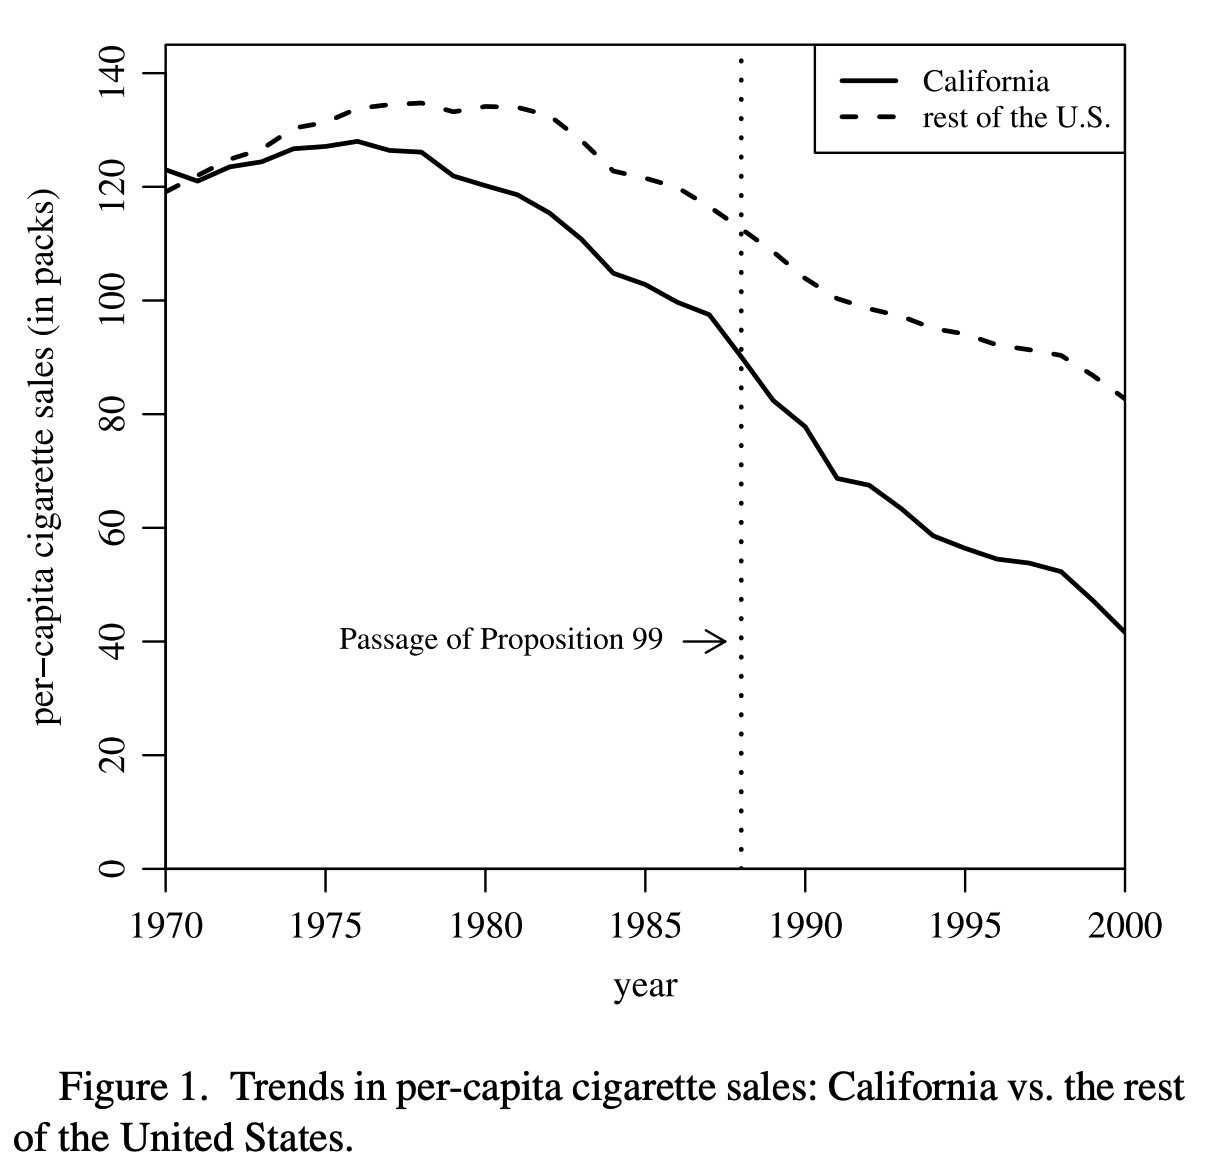
\includegraphics[width=\linewidth]{images/abadie2010a.png}
    \end{column}%
  \end{columns}
\end{frame}


\begin{frame}{Generalized setup (Doudchenko and Imbens (2018))}
  \begin{wideitemize}
  \item Consider the following general problem
    \item We have a panel with $T$ time periods and $N+1$
      units. Intervention $D_{it}$ at time $T_{0}$ for one unit (unit $i = 0$)
    \item Potential outcomes $Y_{it}(D_{it})$, and we only observe one
      of the potential outcomes (as per usual)
      \begin{itemize}
      \item Fundamental problem of causal inference
      \item We can also have fixed characteristics $X_{it}$
      \end{itemize}
    \item Let $\mathbf{Y}_{a,b}$ denote the vector (or matrix in
      control case) for $a \in \{\text{treatment}, \text{control}\}$ and
      $b \in \{\text{pre}, \text{post}\}$ for the treated and control
      groups in the pre or post period.
    \item Then, we have observations (analogous setup for the covariates):
      \begin{equation*}
        \mathbf{Y} = \left( \begin{array}{cc}
                              \mathbf{Y}_{t,post} & \mathbf{Y}_{c,post} \\
                              \mathbf{Y}_{t,pre} & \mathbf{Y}_{c,pre} \\
                            \end{array}
                            \right) =  \left( \begin{array}{cc}
                              \mathbf{Y}_{t,post}(1) & \mathbf{Y}_{c,post}(0) \\
                              \mathbf{Y}_{t,pre}(0) & \mathbf{Y}_{c,pre}(0) \\
                            \end{array}
                            \right) 
      \end{equation*}
  \end{wideitemize}
\end{frame}

\begin{frame}{Generalized panel setup}
      \begin{equation*}
        \mathbf{Y} = \left( \begin{array}{cc}
                              \mathbf{Y}_{t,post} & \mathbf{Y}_{c,post} \\
                              \mathbf{Y}_{t,pre} & \mathbf{Y}_{c,pre} \\
                            \end{array}
                            \right) =  \left( \begin{array}{cc}
                              \mathbf{Y}_{t,post}(1) & \mathbf{Y}_{c,post}(0) \\
                              \mathbf{Y}_{t,pre}(0) & \mathbf{Y}_{c,pre}(0) \\
                            \end{array}
                            \right) 
      \end{equation*}
      \begin{wideitemize}
      \item To estimate $\tau_{i} = Y_{t,post}(1) - Y_{t,post}(0)$, we
        need an estimate for $Y_{t,post}(0)$
      \item What if we just had the cross-section?
        \begin{itemize}
        \item Note that if $D_{it}$ were randomly assigned, we can
          derive an estimate using our p-score or regression methods
        \item Even without random assignment, one could use covariates
          to match
        \item Our main concern with p-score matching is bias
        \end{itemize}
      \item Diff-in-diff exploited the panel structure by asserting a particular functional form
        \begin{equation*}
          Y_{it} = \alpha_{i} + \gamma_{t} + D_{it}\tau + \epsilon_{it}
        \end{equation*}
      \item Is there something particularly special about this linear
        additive factor structure?
      \end{wideitemize}
\end{frame}


\begin{frame}{Generalized panel setup}
      \begin{equation*}
        \mathbf{Y} = \left( \begin{array}{cc}
                              \mathbf{Y}_{t,post} & \mathbf{Y}_{c,post} \\
                              \mathbf{Y}_{t,pre} & \mathbf{Y}_{c,pre} \\
                            \end{array}
                            \right) =  \left( \begin{array}{cc}
                              \mathbf{Y}_{t,post}(1) & \mathbf{Y}_{c,post}(0) \\
                              \mathbf{Y}_{t,pre}(0) & \mathbf{Y}_{c,pre}(0) \\
                            \end{array}
                            \right) 
      \end{equation*}
      \begin{wideitemize}
      \item Recall that our problem boils down to the estimate of an untreated ``synthetic'' unit
      \item Following Doudchenko and Imbens (2018), note estimators of the following form:
        \begin{equation*}
          \hat{Y}_{t,post}(0) = \mu + \sum_{i \in c}\omega_{i} Y_{i, T}
        \end{equation*}
        \begin{itemize}
        \item A constant $\mu$ allows for very different averages (common in diff-in-diff)
        \item Weights are allowed to vary across $i$ -- a simple
          average would be diff-in-diff
        \end{itemize}
      \item We can now consider deviations from diff-in-diff
      \end{wideitemize}
\end{frame}

\begin{frame}{The synthetic control method (Abadie et al. (2010)}
  \begin{columns}[T] % align columns
    \begin{column}{0.8\textwidth}
  \begin{equation*}
    \hat{Y}_{t,post}(0) = \mu + \sum_{i \in c}\omega_{i} Y_{i, T}
  \end{equation*}
  \begin{wideitemize}
  \item In ADH, they impose
    \begin{enumerate}
    \item $\mu = 0$
    \item $\sum_{i} \omega_{i} = 1$
    \item $\omega_{i} \geq 0 \; \forall i$      
    \end{enumerate}
  \item These three restrictions create a counterfactual California
    whose outcomes are within the support of the other states, and
    is a weighted sum of a subset of states
  \end{wideitemize}
\end{column}
\begin{column}{0.4\textwidth}
\end{column}
\end{columns}
\end{frame}

\begin{frame}{The synthetic control method (Abadie et al. (2010)}
  \begin{columns}[T] % align columns
    \begin{column}{0.8\textwidth}
  \begin{equation*}
    \hat{Y}_{t,post}(0) = \mu + \sum_{i \in c}\omega_{i} Y_{i, T}
  \end{equation*}
  \begin{wideitemize}
  \item Formally, the $\omega_{i}$ need to be estimated, and are
    constructed by minimizing the distance between covariates in the pre-period:
    \begin{equation*}
      ||\boldsymbol{X}_{\text{treat}} - \boldsymbol{X}_{\text{control}}\boldsymbol{W}||
    \end{equation*}
  \item The crucial piece tying this together: $\boldsymbol{X}$ can
    include both lagged outcomes, and covariates.
  \item Note we can now re-envision our panel data:
    \begin{itemize}
    \item Observed outcomes:     $\mathbf{Y}_{t,post}(1)$, $\mathbf{Y}_{c,post}(0)$
    \item Observed covariates / predictors: $\mathbf{Y}_{t,pre}(0)$, $\mathbf{Y}_{c,pre}(0)$, $\mathbf{X}_{t}$, $\mathbf{X}_{c}$
    \end{itemize}
  \item In many ways, this is just a matching problem using many characteristics!
  \end{wideitemize}
\end{column}
\begin{column}{0.4\textwidth}
\end{column}
\end{columns}
\end{frame}

\begin{frame}{The synthetic control method (Abadie et al. (2010)}
  \begin{columns}[T] % align columns
    \begin{column}{0.9\textwidth}
  \begin{equation*}
    \hat{Y}_{t,post}(0) = \mu + \sum_{i \in c}\omega_{i} Y_{i, T}
  \end{equation*}
  \begin{wideitemize}
  \item Formally, the $\omega_{i}$ need to be estimated, and are
    constructed by minimizing the distance between covariates in the pre-period:
    \begin{equation*}
      \{\hat{\omega} \}_{i} = \arg\min_{\boldsymbol{W}}||\boldsymbol{X}_{\text{treat}} - \boldsymbol{X}_{\text{control}}\boldsymbol{W}||
    \end{equation*}
  \item The crucial piece tying this together: $\boldsymbol{X}$ can
    include both lagged outcomes, and covariates.
  \item Note we can now re-envision our panel data:
    \begin{itemize}
    \item Observed outcomes:     $\mathbf{Y}_{t,post}(1)$, $\mathbf{Y}_{c,post}(0)$
    \item Observed covariates / predictors: $\mathbf{Y}_{t,pre}(0)$, $\mathbf{Y}_{c,pre}(0)$, $\mathbf{X}_{t}$, $\mathbf{X}_{c}$
    \end{itemize}
  \item In many ways, this is just a matching problem using many characteristics!
  \end{wideitemize}
\end{column}
\begin{column}{0.4\textwidth}
\end{column}
\end{columns}
\end{frame}

\begin{frame}{The synthetic control method (Abadie et al. (2010)}
  \begin{columns}[T] % align columns
    \begin{column}{0.5\textwidth}
  \begin{wideitemize}
  \item<1-> This approach can be incredibly successful
  \item<2-> By careful construction of a synthetic control, can
    calculate counterfactual impacts due to policy
  \item<2-> Still subject to same caveats from DinD -- not invariant
    to some transformations (e.g. log and linear)
  \end{wideitemize}
\end{column}
\begin{column}{0.5\textwidth}
  \only<1>{  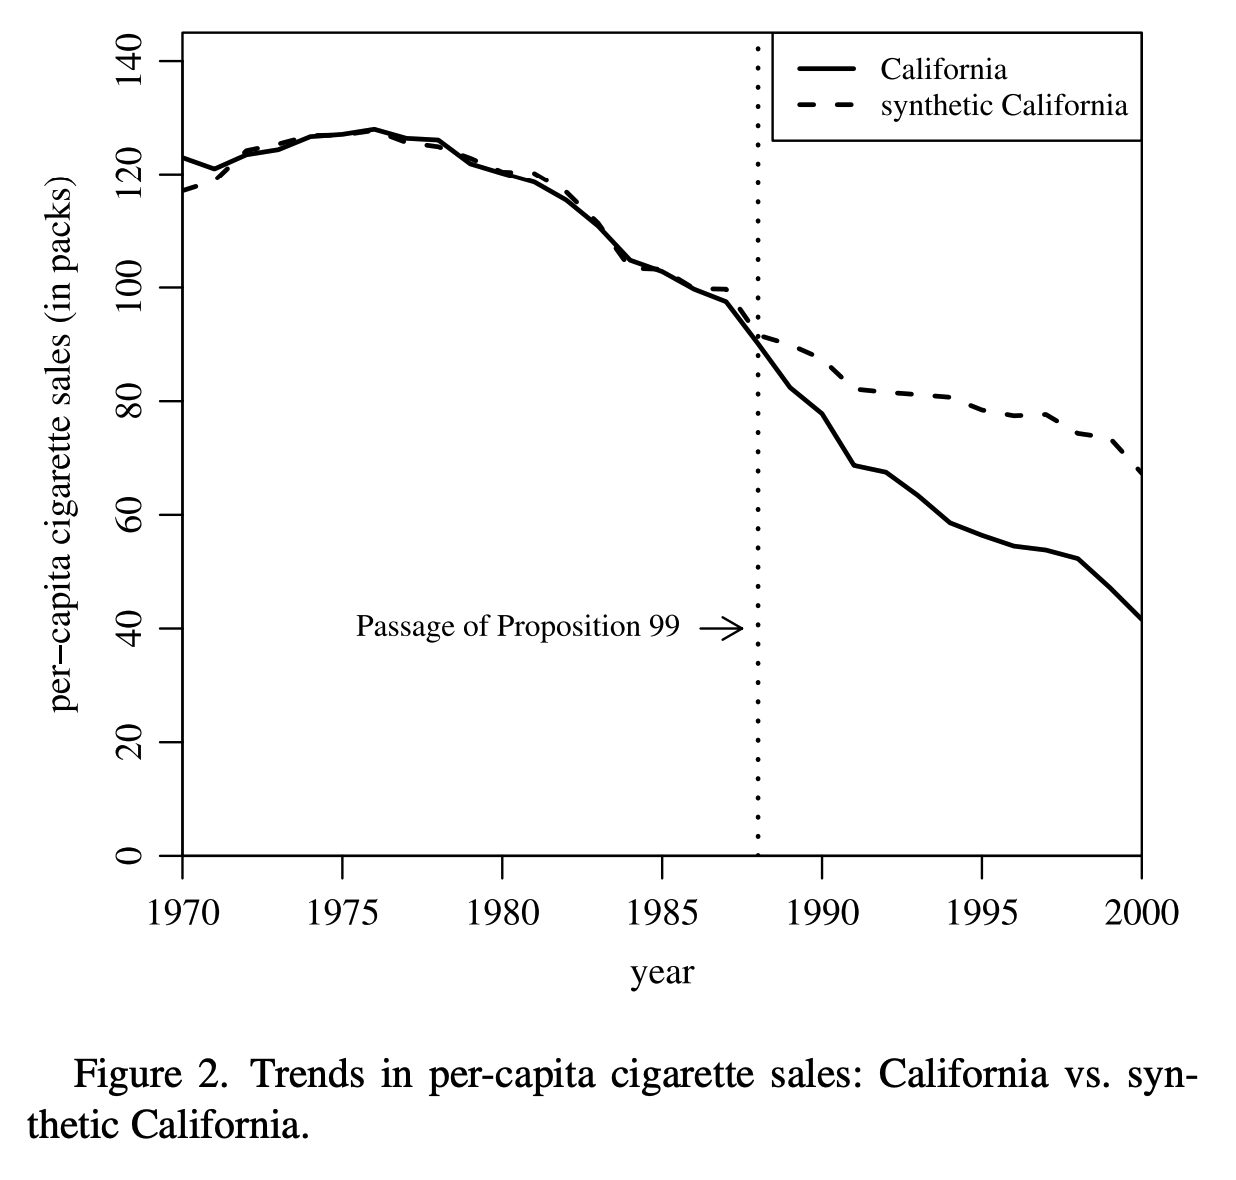
\includegraphics[width=\linewidth]{images/abadie2010b.png}}
\only<2>{  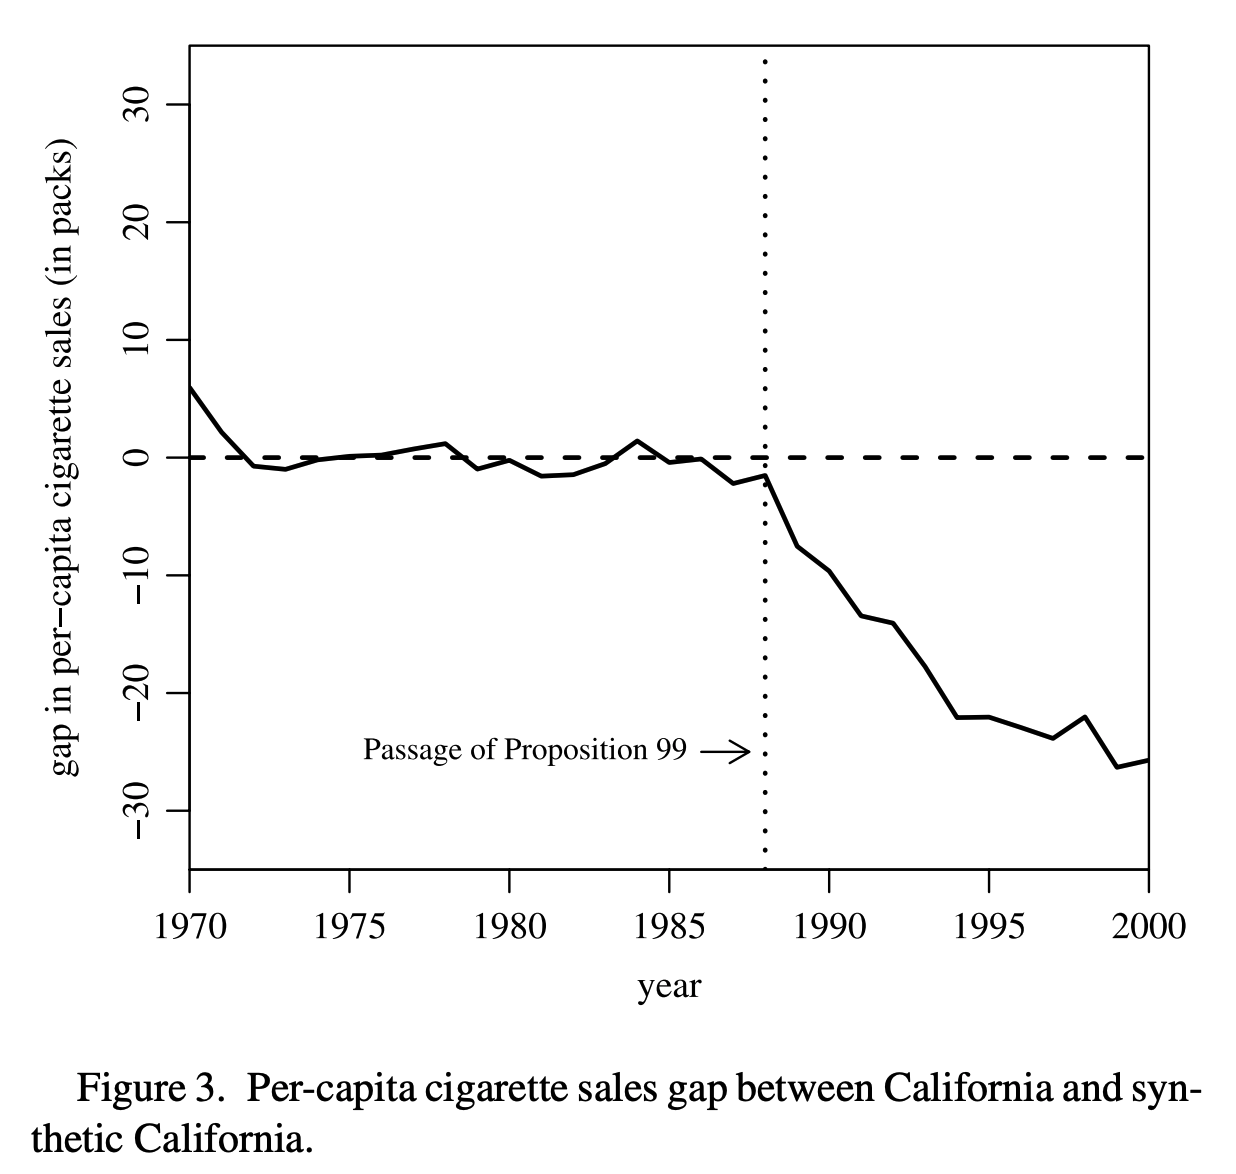
\includegraphics[width=\linewidth]{images/abadie2010c.png}}  
\end{column}
\end{columns}
\end{frame}


\begin{frame}{Inference in the synthetic control method (Abadie et al. (2010)}
  \begin{columns}[T] % align columns
    \begin{column}{0.5\textwidth}
  \begin{wideitemize}
  \item Inference for this method is slightly more complex, as there
    is only a single treated unit
    \begin{itemize}
    \item Large sample asymptotics unlikely to work
    \end{itemize}
  \item Placebo approach is standard: apply method to each potential
    control unit, and report effect in period
  \item Analogy here is to a randomization inference argument,
    comparing to a ``null'' effect
  \end{wideitemize}
\end{column}
\begin{column}{0.5\textwidth}
  \only<1>{  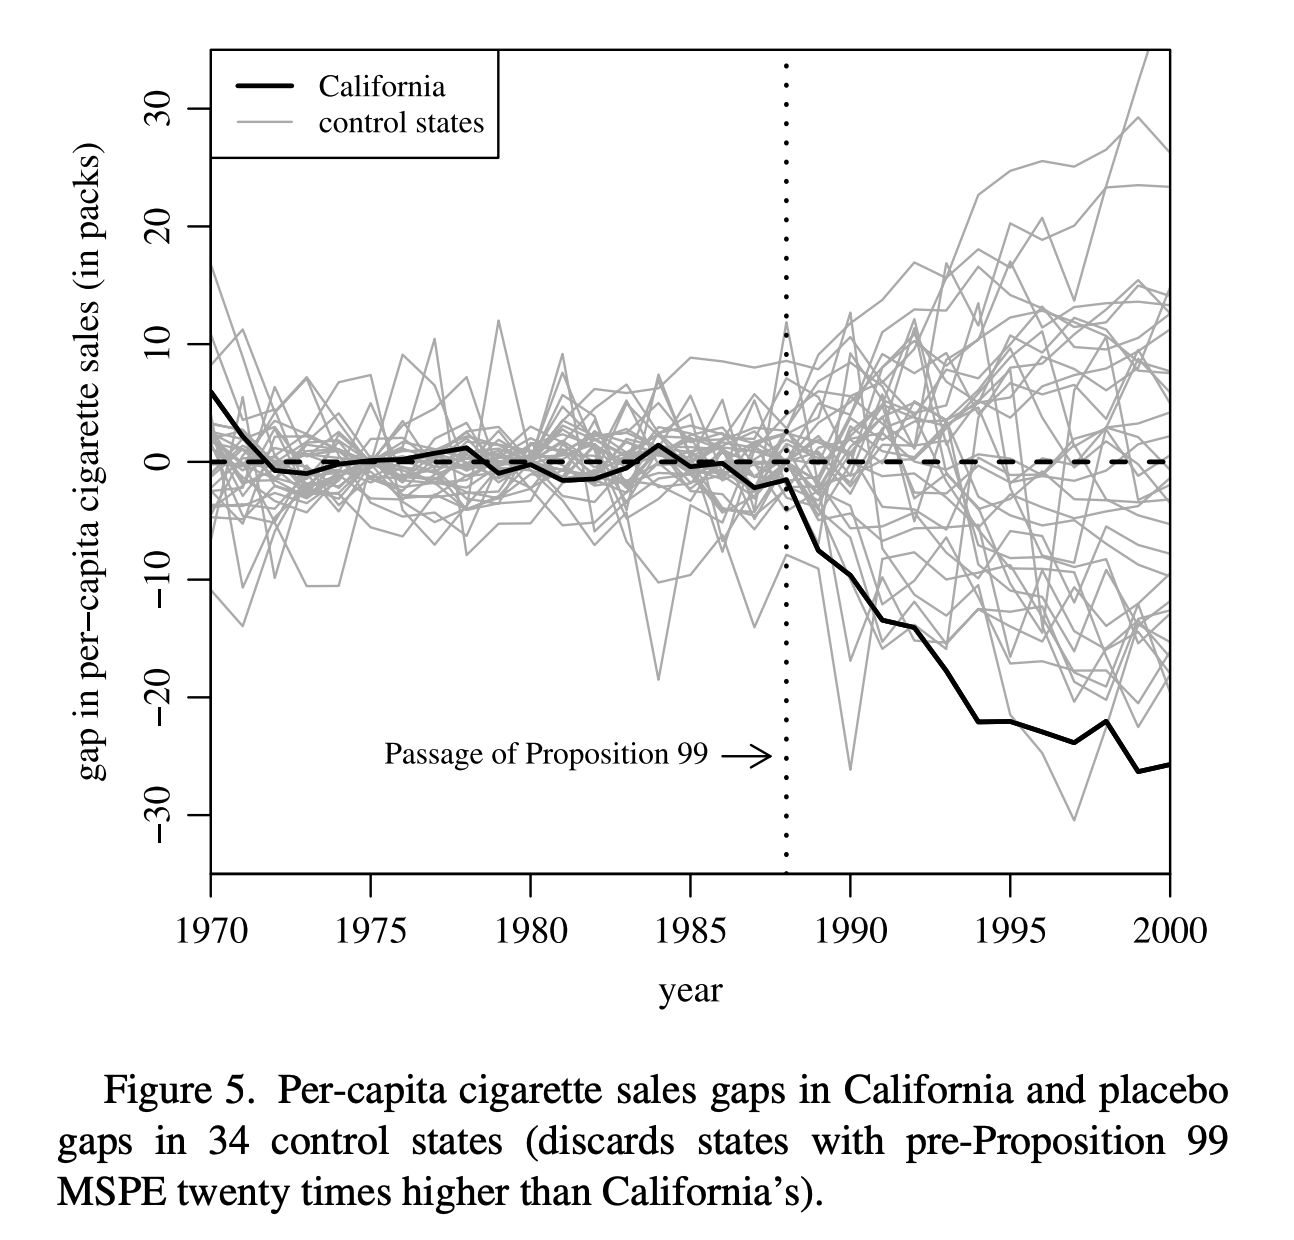
\includegraphics[width=\linewidth]{images/abadie2010d.png}}
\end{column}
\end{columns}
\end{frame}

\begin{frame}{Synthetic Diff-in-diff}
  \begin{wideitemize}
  \item In Arkhangelsky et al. (2019), they show you can rewrite the synthetic control estimator as 
    \begin{equation*}
      (\hat{\mu}, \hat{\gamma}, \hat{\tau}) = \arg\min_{\mu, \gamma, \tau}\sum_{i}\sum_{t}(Y_{it} - \mu - \gamma_{t} - D_{it}\tau)^{2}\hat{\omega}_{i},
    \end{equation*}
    subject to the $\hat{\omega}_{i}$ chosen via the SC approach
  \item Contrast that with DID:
    \begin{equation*}
      (\hat{\mu},\hat{\alpha}, \hat{\gamma}, \hat{\tau}) = \arg\min_{\mu, \gamma, \tau}\sum_{i}\sum_{t}(Y_{it} - \mu -\alpha_{i} - \gamma_{t} - D_{it}\tau)^{2}
    \end{equation*}
  \item They then propose a more robust approach, called Synthetic diff-in-diff, which estimates
    \begin{equation*}
      (\hat{\mu},\hat{\alpha}, \hat{\gamma}, \hat{\tau}) = \arg\min_{\mu, \gamma, \tau}\sum_{i}\sum_{t}(Y_{it} - \mu -\alpha_{i} - \gamma_{t} - D_{it}\tau)^{2}\hat{\omega}_{i}\hat{\lambda}_{t}
    \end{equation*}
  \item This approach relaxes the parallel trends assumption by requiring parallel trends in an underlying approximate factor structure
  \end{wideitemize}
\end{frame}

\begin{frame}{Synthetic Diff-in-diff}
  \begin{columns}[T] % align columns
    \begin{column}{0.5\textwidth}
  \begin{wideitemize}
  \item Key difference is twofold:
    \begin{enumerate}
    \item Pre-trend means do not need to match ``exactly''
    \item Weighting is not equivalent across all time periods
    \end{enumerate}
  \item Conceptually -- different ways to generate the counterfactual given a model 
  \end{wideitemize}
\end{column}
\begin{column}{0.5\textwidth}
  \only<1>{  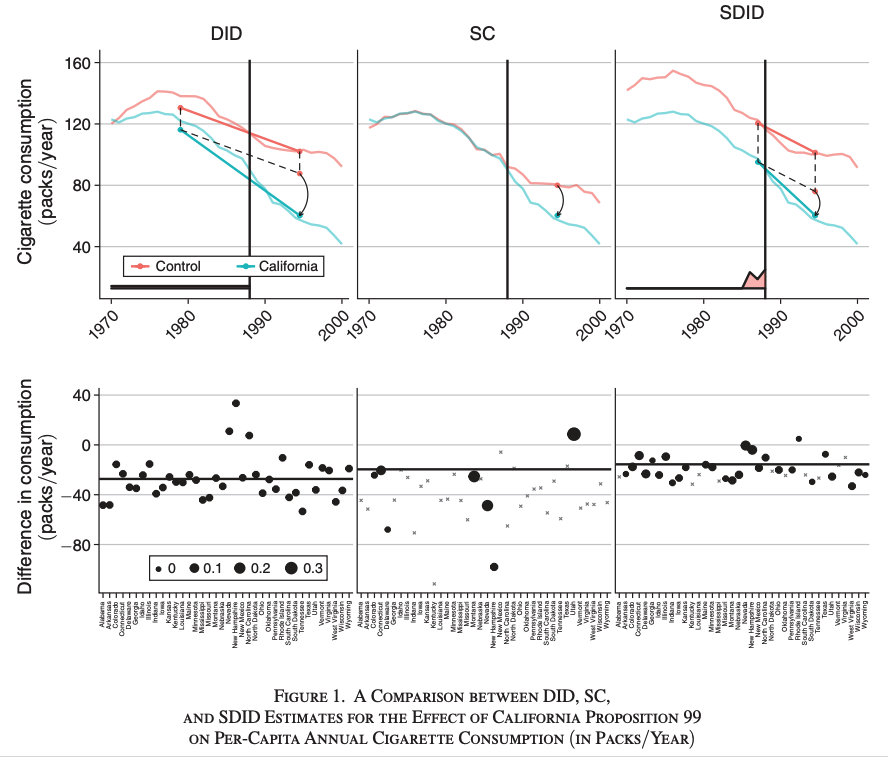
\includegraphics[width=\linewidth]{images/synthdid.png}}
  \only<2>{  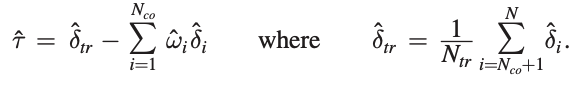
\includegraphics[width=\linewidth]{images/synthdid_eq1.png}\\
     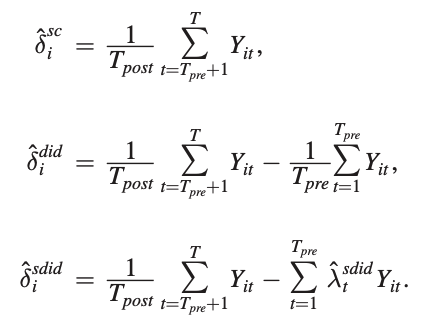
\includegraphics[width=\linewidth]{images/synth_eq2.png}} 
\end{column}
\end{columns}
\end{frame}

\begin{frame}{Synthetic Diff-in-diff}
  \begin{columns}[T] % align columns
    \begin{column}{0.5\textwidth}
  \begin{wideitemize}
  \item So far, synth dind method discussion focused on single adoption period. 
    \begin{enumerate}
    \item Staggered adoption in synthetic control isn't meaningful
    \item How can you adopt it?
    \end{enumerate}
  \item Conceptually -- split up the adoption timings a la Calloway \& Sant'anna and others
  \end{wideitemize}
\end{column}
\begin{column}{0.5\textwidth}
  \only<1>{  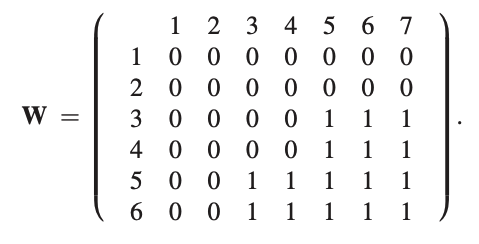
\includegraphics[width=\linewidth]{images/synthdid_staggered1.png}}
  \only<2>{  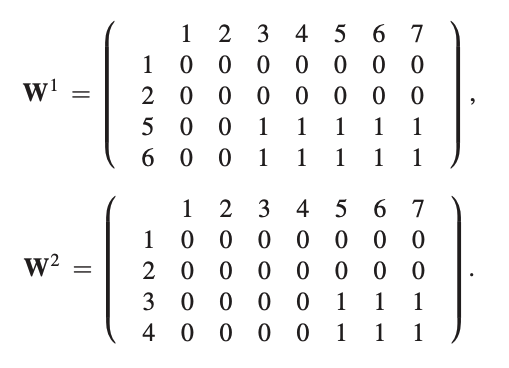
\includegraphics[width=\linewidth]{images/synthdid_staggered2.png}}
\end{column}
\end{columns}
\end{frame}


\begin{frame}{So what about synthetic methods?}
  \begin{wideitemize}
  \item Both an old field, and a new one -- lots of new methodological papers coming out 
    \begin{itemize}
    \item It is a very cool method!
    \end{itemize}
  \item So far, limited application by researchers. Why?
  \item  My thoughts:
    \begin{itemize}
    \item These are strong structural assumptions, and not clear we
      have good tests yet
    \item Despite concerns re: pre-trends in dind, the assumptions
      felt testable
    \end{itemize}
  \item Researcher degrees of freedom seem multifold. True in DinD
    too, but perhaps more transparent?
    \begin{itemize}
    \item More worrisome: dind is equally problematic, but we aren't
      aware of it
    \end{itemize}
  \item If researchers are more willing to understand that DinD is
    sensitive to functional form, ML methods that construct
    counterfactual outcomes are a natural direction
  \end{wideitemize}
\end{frame}



\begin{frame}{My recommendation / takeaway}
  \begin{wideitemize}
  \item Synthetic control is the ideal approach when faced with a single treatment
    \begin{itemize}
    \item By far the most natural approach in this setting, and is a practical approach
    \item Typcial approach -- get a good synthetic control for a given
      treatment. If none exists, stop. Ben-Michael, Feller and
      Rothstein (2021) provide a better approach, which adjusts for
      imperfect pre-match.
    \end{itemize}
  \item Synthetic DiD seems very promising as a generalization
    \begin{itemize}
    \item Key question is convincing readers why this shoudl work better than traditional method
    \item My view: empirical papers will first need to show how / why
      their method works with both diff-in-diff and synth diff-in-diff
    \end{itemize}
  \item Key point: \emph{all of this relies on a model of the control outcome}
  \item Three packages to explore: augsynth/tidysynth andsynthdid
    packages (original synth package is tough to use)
  \end{wideitemize}
\end{frame}

\begin{frame}{Next class}
  \begin{wideitemize}
    \item Extensions: continuous treatments, multiple treatments,
      alternative approaches
    \item Checklist: What do you need to do?
    \end{wideitemize}
\end{frame}

\end{document}
